\chapter{Resultados}
\label{chap:resultados}

Este capítulo apresenta os resultados do experimento fatorial descrito na
Seção~\ref{sec:fatorial}. A Seção~\ref{sec:res_detector} descreve o
comportamento do detector, comum a todas as condições; as
Seções~\ref{sec:res_eficacia} a~\ref{sec:res_sensibilidade} respondem à
questão principal; e a Seção~\ref{sec:res_derivada} apresenta os resultados
da questão derivada. Todas as médias referem-se a dez repetições por
condição, salvo indicação em contrário, e todas as acurácias são acurácias
prequential calculadas a partir do início do drift. O notebook que produz
cada tabela e figura está disponível no repositório do trabalho.

\section{Comportamento do Detector}
\label{sec:res_detector}

Antes de comparar as estratégias, é preciso caracterizar o detector que
aciona três delas. A Tabela~\ref{tab:deteccao} resume o desempenho do HDDDM
por tipo e severidade. Das 180 transições injetadas nas 120 streams, 136
(75,6\%) foram detectadas dentro da janela de tolerância. A taxa de detecção
cresce com a severidade, de 60\% na severidade baixa para 82\% na média e
85\% na alta, e é menor nos padrões lentos: 63\% no gradual e 73\% no
incremental, contra 83\% no abrupto e 78\% no recorrente. Nos padrões
abrupto e recorrente, toda detecção ocorre no próprio bloco da mudança; nos
padrões gradual e incremental, a detecção ocorre em média entre 0,7 e 4
blocos após o início da transição, isto é, ainda durante ela. Antes do
drift, o detector produziu 0,028 falso alarme por bloco.

\begin{table}[htbp]
\centering
\small
\caption{Desempenho do HDDDM por tipo e severidade do drift}
\label{tab:deteccao}
\begin{adjustbox}{max width=\textwidth}
\begin{tabular}{llrrrr}
\toprule
Tipo & Severidade & Taxa de detecção & Atraso (blocos) & Detecções/stream & Falsos alarmes pré-drift \\
\midrule
Abrupto & Baixa & 0,600 & 0,000 & 2,000 & 0,800 \\
 & Média & 0,900 & 0,000 & 1,800 & 0,300 \\
 & Alta & 1,000 & 0,000 & 2,100 & 0,400 \\
Gradual & Baixa & 0,400 & 4,000 & 1,400 & 0,600 \\
 & Média & 0,600 & 1,500 & 1,400 & 0,300 \\
 & Alta & 0,900 & 0,667 & 2,500 & 0,200 \\
Incremental & Baixa & 0,600 & 2,833 & 1,300 & 0,300 \\
 & Média & 0,700 & 1,429 & 1,800 & 0,700 \\
 & Alta & 0,900 & 1,889 & 1,600 & 0,200 \\
Recorrente & Baixa & 0,667 & 0,000 & 3,500 & 0,400 \\
 & Média & 0,900 & 0,000 & 3,500 & 0,000 \\
 & Alta & 0,767 & 0,000 & 3,500 & 0,300 \\
\bottomrule
\end{tabular}
\end{adjustbox}
\end{table}


A severidade observada pelo detector converge para a severidade real à
medida que a janela cresce (Figura~\ref{fig:convergencia}). Com blocos de 400
instâncias, o valor estimado entre duas amostras da mesma distribuição fica
em torno de 0,055, o que define um piso de ruído amostral; o limiar de
recorrência derivado desse ruído (Seção~\ref{sec:config_detector}) foi
$\theta = 0{,}073$.

\begin{figure}[htbp]
\centering
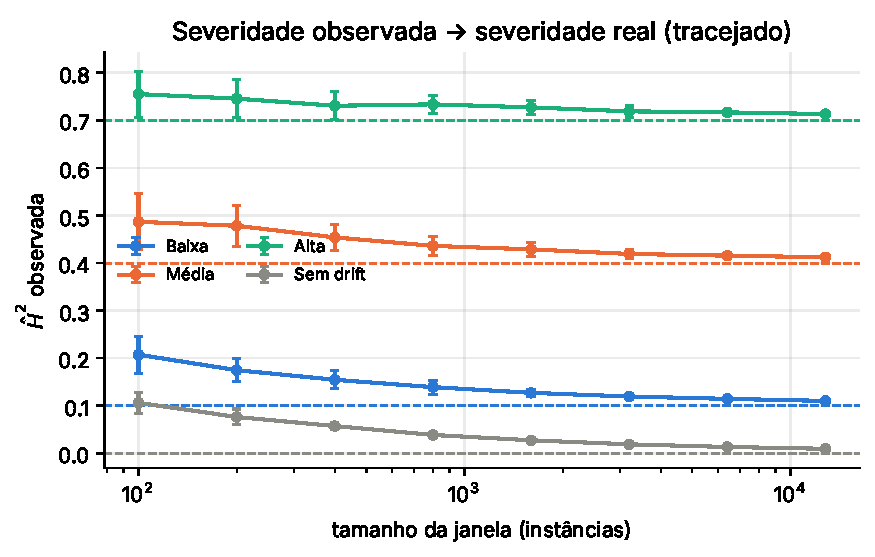
\includegraphics[width=0.75\textwidth]{figuras/resultados/fig_convergencia_severidade.pdf}
\caption{Severidade observada ($\hat{H}^2$) em função do tamanho da janela,
para cada nível de severidade real (linhas tracejadas) e para duas amostras
sem drift. Barras: desvio-padrão em 60 sorteios.}
\label{fig:convergencia}
\end{figure}

\section{Eficácia das Estratégias}
\label{sec:res_eficacia}

A acurácia média antes do drift foi de 0,891. Após o drift, considerando
todas as condições, a janela deslizante obteve a maior acurácia média
(0,860), seguida do reset completo (0,805) e da reativação de modelos
históricos (0,804), praticamente empatados, do retreinamento incremental
(0,749) e da condição de controle (0,655). Todas as estratégias superaram o
controle. A Figura~\ref{fig:heatmap} detalha a acurácia de cada estratégia
nas 36 combinações de tipo, severidade e classificador, e as
Tabelas~\ref{tab:acc-naivebayes} a~\ref{tab:acc-xgboost}, no
Apêndice~\ref{ap:tabelas}, trazem os mesmos valores por classificador.

\begin{figure}[htbp]
\centering
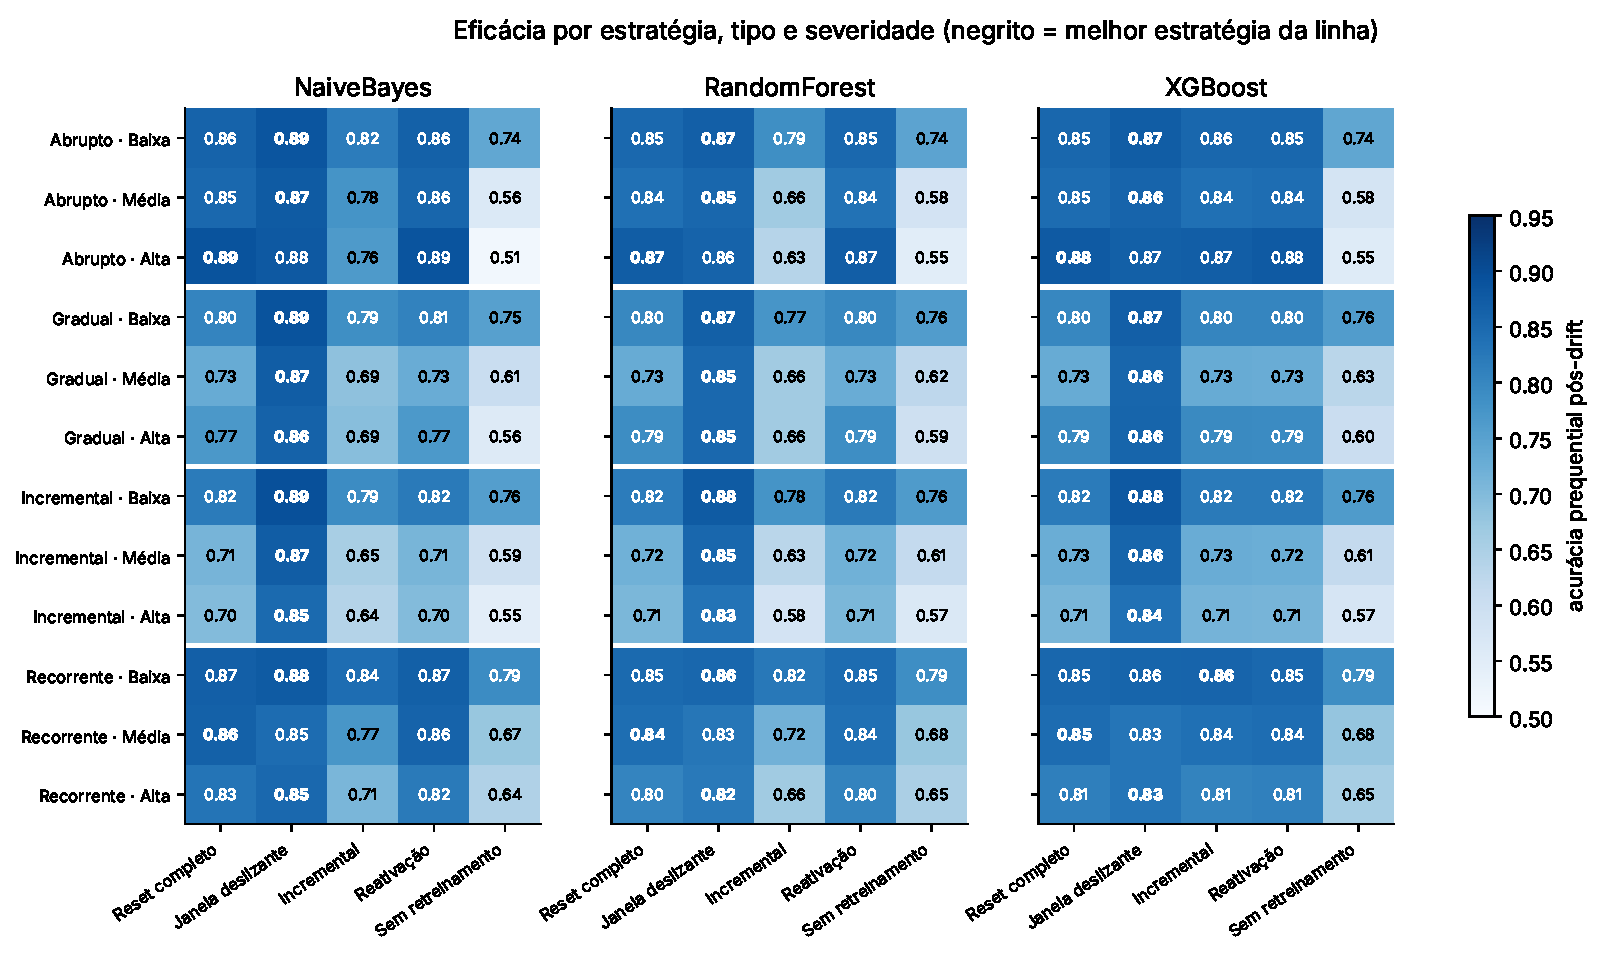
\includegraphics[width=\textwidth]{figuras/resultados/fig_heatmap_eficacia.pdf}
\caption{Acurácia prequential pós-drift média por estratégia, tipo e
severidade, para cada classificador. Em negrito, a melhor estratégia de
cada linha, excluído o controle.}
\label{fig:heatmap}
\end{figure}

A janela deslizante foi a melhor estratégia em 29 das 36 combinações. As
exceções concentram-se em dois casos: o drift abrupto de severidade alta,
no qual o reset completo foi a melhor estratégia para os três
classificadores, e o drift recorrente de severidade média, no qual o reset
também superou a janela para os três classificadores; além disso, com o
XGBoost, o retreinamento incremental foi o melhor sob drift recorrente de
severidade baixa. Em todas as exceções, as diferenças em relação à janela
são pequenas, de no máximo 0,018.

\subsection{Efeito do tipo de drift}

O tipo de drift alterou sobretudo a distância entre a janela deslizante e
as estratégias acionadas por detecção. Nos padrões abrupto e recorrente, a
vantagem média da janela sobre o reset completo foi de apenas 0,009 e 0,003,
respectivamente; nos padrões gradual e incremental, chegou a 0,093 e 0,114.
A Figura~\ref{fig:curvas} mostra a origem dessa diferença. Sob drift
abrupto, o reset, a reativação e a janela recuperam o desempenho em poucos
blocos. Sob drift gradual e incremental, as estratégias reativas retreinam
assim que o HDDDM sinaliza a mudança, ainda no início da transição; o modelo
resultante é treinado sobre uma distribuição intermediária e, como o
detector costuma disparar uma única vez durante a transição (em 31 das 42
streams lentas com alguma detecção nesse intervalo), esse modelo permanece em
uso depois que a transição termina. A
janela deslizante, por retreinar em cadência fixa, acompanha a transição até
o fim.

\begin{figure}[htbp]
\centering
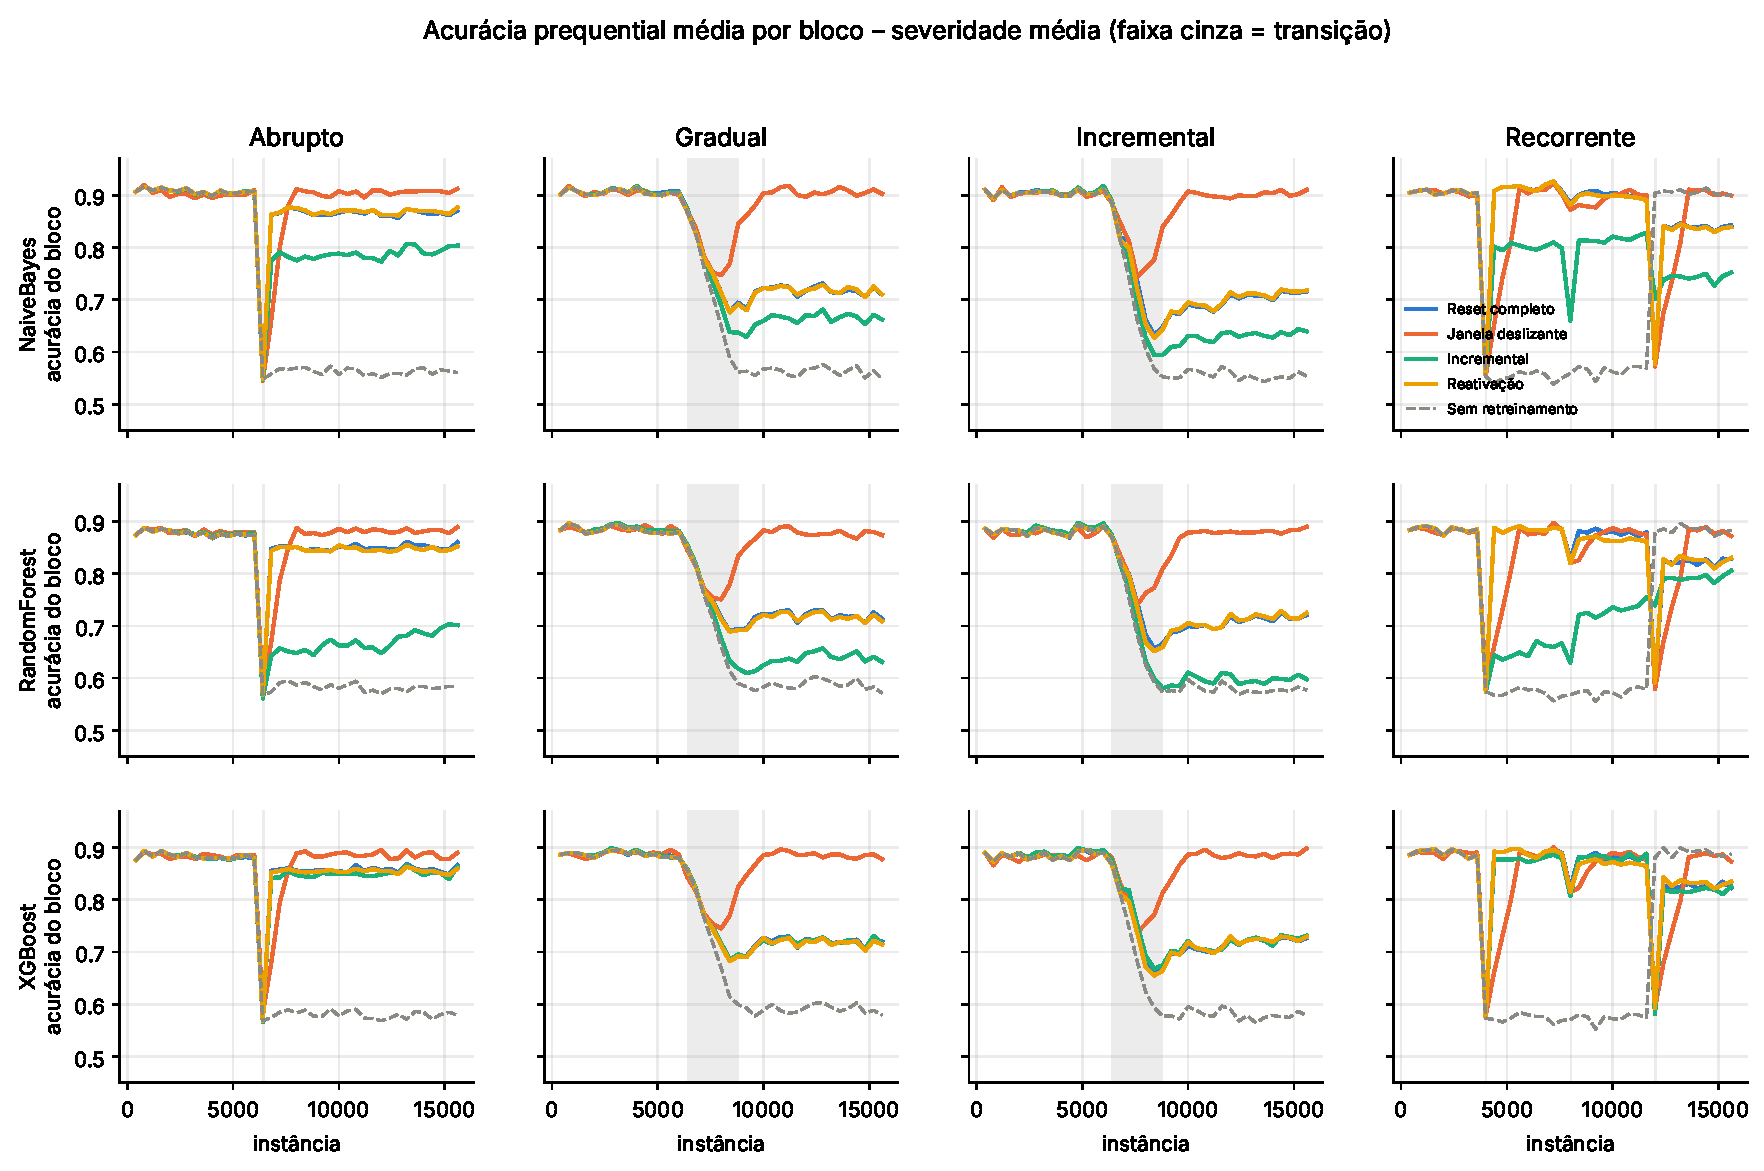
\includegraphics[width=\textwidth]{figuras/resultados/fig_curvas_prequential.pdf}
\caption{Acurácia prequential média por bloco, sob severidade média, para
cada classificador e tipo de drift. A faixa cinza marca a janela de
transição dos padrões gradual e incremental.}
\label{fig:curvas}
\end{figure}

Sob drift recorrente, a reativação de modelos históricos não superou o reset
completo (0,838 contra 0,841). No retorno ao estado inicial, o repositório
identificou corretamente o modelo treinado sob $P$, mas esse modelo, treinado
sobre um único bloco de $P$, não é melhor que um modelo novo treinado sobre
outro bloco da mesma distribuição. Nas condições deste experimento, a
vantagem da reativação limita-se, portanto, ao custo, discutido na
Seção~\ref{sec:res_custo}.

\subsection{Efeito da severidade}

A severidade ampliou o ganho de todas as estratégias sobre o controle, já
que o modelo não atualizado se degrada mais quanto maior o deslocamento
(Figura~\ref{fig:ganho}). Sob severidade baixa, o ganho médio sobre o
controle foi de 0,112 para a janela deslizante e de 0,071 para o reset
completo; sob severidade alta, de 0,266 e 0,212. A ordenação entre as
estratégias, no entanto, pouco mudou com a severidade: a janela teve o maior
ganho nos três níveis, e o reset só a superou no drift abrupto de severidade
alta e no recorrente de severidade média. O retreinamento incremental teve o menor ganho em
todos os níveis, e sua desvantagem cresceu com a severidade.

\begin{figure}[htbp]
\centering
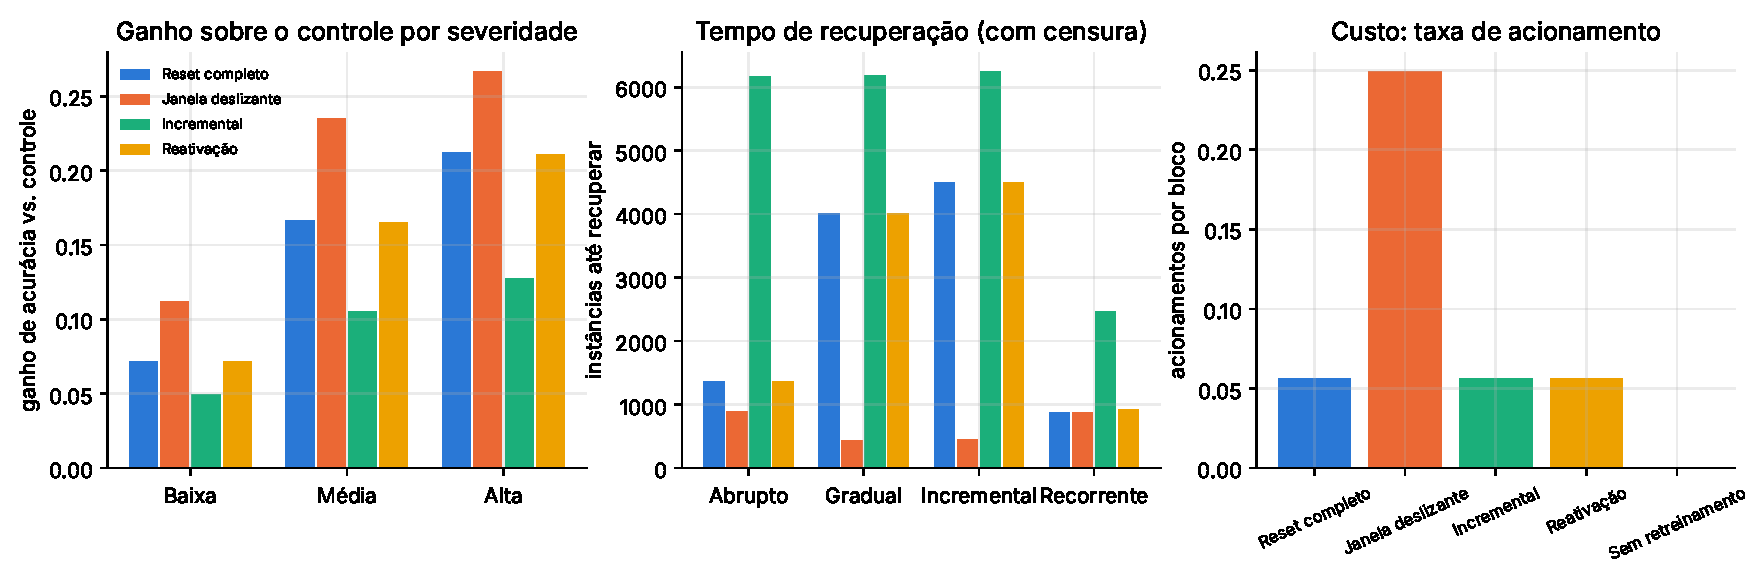
\includegraphics[width=\textwidth]{figuras/resultados/fig_ganho_recuperacao_custo.pdf}
\caption{Ganho médio de acurácia sobre o controle por severidade (esquerda),
tempo médio de recuperação por tipo de drift, com censura no fim de cada
segmento (centro), e taxa média de acionamento por estratégia (direita).}
\label{fig:ganho}
\end{figure}

\subsection{Efeito do classificador}

O classificador alterou principalmente a eficácia do retreinamento
incremental. Com o XGBoost, cuja atualização acrescenta novas rodadas de
boosting que corrigem o conjunto existente, o incremental atingiu acurácia
pós-drift média de 0,805, equivalente à do reset completo (0,806). Com o
Naive Bayes, cuja atualização acumula estatísticas antigas e novas, o
incremental ficou em 0,744; com o Random Forest, cuja atualização acrescenta
árvores novas a uma maioria de árvores treinadas antes do drift, ficou em
0,698. Para as demais estratégias, a diferença entre classificadores foi
pequena: a janela deslizante variou entre 0,852 e 0,871 e o reset, entre
0,801 e 0,808.

\section{Análise Estatística}
\label{sec:res_estatistica}

A Tabela~\ref{tab:anova} apresenta a ANOVA em parcelas subdivididas. A
estratégia foi o fator de maior efeito ($\eta^2_p = 0{,}783$), seguida da
severidade (0,439), das interações tipo $\times$ estratégia (0,323) e
severidade $\times$ estratégia (0,311), do tipo (0,308) e da interação
classificador $\times$ estratégia (0,189). As três interações com a
estratégia confirmam que a eficácia relativa das estratégias depende do tipo
e da severidade do drift e do classificador. A interação tripla tipo
$\times$ severidade $\times$ estratégia também foi significativa, mas com
efeito menor (0,090), e as interações de quarta ordem e tipo $\times$
severidade $\times$ classificador não foram significativas.

\begin{table}[htbp]
\centering
\small
\caption{ANOVA em parcelas subdivididas da acurácia prequential pós-drift}
\label{tab:anova}
\begin{adjustbox}{max width=\textwidth}
\begin{tabular}{llrrrr}
\toprule
Termo & Estrato & gl & F & $p$ & $\eta^2_p$ \\
\midrule
Estratégia & Dentro & 4; 1512 & 1365,20 & $<$ 0,001 & 0,783 \\
Severidade & Entre & 2; 108 & 42,25 & $<$ 0,001 & 0,439 \\
Tipo $\times$ Estratégia & Dentro & 12; 1512 & 60,00 & $<$ 0,001 & 0,323 \\
Severidade $\times$ Estratégia & Dentro & 8; 1512 & 85,46 & $<$ 0,001 & 0,311 \\
Tipo & Entre & 3; 108 & 16,04 & $<$ 0,001 & 0,308 \\
Classificador $\times$ Estratégia & Dentro & 8; 1512 & 44,05 & $<$ 0,001 & 0,189 \\
Tipo $\times$ Severidade & Entre & 6; 108 & 2,43 & 0,030 & 0,119 \\
Tipo $\times$ Severidade $\times$ Estratégia & Dentro & 24; 1512 & 6,23 & $<$ 0,001 & 0,090 \\
Classificador & Dentro & 2; 1512 & 56,08 & $<$ 0,001 & 0,069 \\
Severidade $\times$ Classificador $\times$ Estratégia & Dentro & 16; 1512 & 4,20 & $<$ 0,001 & 0,043 \\
Tipo $\times$ Classificador $\times$ Estratégia & Dentro & 24; 1512 & 1,67 & 0,023 & 0,026 \\
Severidade $\times$ Classificador & Dentro & 4; 1512 & 6,73 & $<$ 0,001 & 0,017 \\
Tipo $\times$ Classificador & Dentro & 6; 1512 & 3,42 & 0,002 & 0,013 \\
Tipo $\times$ Severidade $\times$ Classificador $\times$ Estratégia & Dentro & 48; 1512 & 0,25 & 1,000 & 0,008 \\
Tipo $\times$ Severidade $\times$ Classificador & Dentro & 12; 1512 & 0,63 & 0,815 & 0,005 \\
\bottomrule
\end{tabular}
\end{adjustbox}
\par\vspace{2pt}{\footnotesize gl: graus de liberdade do efeito e do erro. Entre: efeitos testados contra a variação entre streams (120 streams); dentro: contra a variação residual dentro das streams.}
\end{table}


Os testes não paramétricos confirmam a ordenação. O teste de Friedman,
tomando as 120 streams como blocos, rejeitou a igualdade entre as
estratégias ($\chi^2 = 325{,}1$; $p < 0{,}001$), com rank médio de 1,77 para
a janela deslizante, 2,22 para o reset completo, 2,37 para a reativação,
3,90 para o incremental e 4,74 para o controle. Nas comparações par a par
(Tabela~\ref{tab:wilcoxon}), todas as diferenças foram significativas após a
correção de Holm, exceto entre o reset completo e a reativação ($p = 0{,}118$).

\begin{table}[htbp]
\centering
\small
\caption{Comparações par a par entre estratégias (teste de Wilcoxon pareado, correção de Holm)}
\label{tab:wilcoxon}
\begin{tabular}{llrr}
\toprule
Estratégia A & Estratégia B & Mediana (A $-$ B) & $p$ (Holm) \\
\midrule
Reset completo & Janela deslizante & -0,008 & $<$ 0,001 \\
Reset completo & Incremental & 0,052 & $<$ 0,001 \\
Reset completo & Reativação & 0,000 & 0,118 \\
Reset completo & Sem retreinamento & 0,134 & $<$ 0,001 \\
Janela deslizante & Incremental & 0,099 & $<$ 0,001 \\
Janela deslizante & Reativação & 0,011 & $<$ 0,001 \\
Janela deslizante & Sem retreinamento & 0,219 & $<$ 0,001 \\
Incremental & Reativação & -0,052 & $<$ 0,001 \\
Incremental & Sem retreinamento & 0,081 & $<$ 0,001 \\
Reativação & Sem retreinamento & 0,134 & $<$ 0,001 \\
\bottomrule
\end{tabular}
\par\vspace{2pt}{\footnotesize Blocos pareados: as 120 streams (acurácia média dos três classificadores). Friedman: $\chi^2$ = 325,1, $p$ $<$ 0,001.}
\end{table}


\section{Custo e Recuperação}
\label{sec:res_custo}

A vantagem da janela deslizante tem um custo (Tabela~\ref{tab:custo}). Com
cadência de quatro blocos, a janela retreinou 9,7 vezes por stream, contra
2,2 vezes do reset completo, e seu tempo total de treino foi cerca de 4,4
vezes maior (0,235~s contra 0,054~s por stream, em média; por serem medidos
em tempo de relógio, esses valores variam ligeiramente entre execuções). Em
contrapartida, foi a única estratégia que recuperou a acurácia pré-drift em
todas as transições, em média 659 instâncias após o fim da transição. O
reset completo recuperou em 67,9\% das transições: em 90\% das transições
abruptas, mas em apenas 50\% das graduais e 46\% das incrementais. O
retreinamento incremental recuperou em 32,0\%.

A reativação teve o menor custo entre as estratégias reativas, com 1,2
treinos e 1,0 reativação por stream. Das reativações, no entanto, 0,8 por
stream ocorreram após alarmes falsos, quando o modelo escolhido era o
próprio modelo em uso e nenhuma troca de fato aconteceu; as reativações
efetivas concentraram-se nos retornos do padrão recorrente.

\begin{table}[htbp]
\centering
\small
\caption{Custo e recuperação por estratégia (média sobre todas as condições)}
\label{tab:custo}
\begin{adjustbox}{max width=\textwidth}
\begin{tabular}{lrrrrrrr}
\toprule
Estratégia & Acion./bloco & Treinos & Reativações & \quad após alarme falso & Treino (s) & Recuperação (inst.) & Recuperou (\%) \\
\midrule
Reset completo & 0,056 & 2,2 & 0,0 & 0,0 & 0,054 & 2.688 & 67,9 \\
Janela deslizante & 0,249 & 9,7 & 0,0 & 0,0 & 0,235 & 659 & 100,0 \\
Incremental & 0,056 & 2,2 & 0,0 & 0,0 & 0,030 & 5.264 & 32,0 \\
Reativação & 0,056 & 1,2 & 1,0 & 0,8 & 0,029 & 2.700 & 67,5 \\
Sem retreinamento & 0,000 & 0,0 & 0,0 & 0,0 & 0,000 & 6.667 & 8,3 \\
\bottomrule
\end{tabular}
\end{adjustbox}
\par\vspace{2pt}{\footnotesize Reativações após alarme falso: o candidato escolhido era o próprio modelo corrente, isto é, não houve mudança de modelo. Recuperação: instâncias após o fim da transição até a acurácia do bloco voltar a até 3 p.p. da acurácia pré-drift (censurada no fim do segmento).}
\end{table}


\section{Efeito do Detector}
\label{sec:res_detector_ideal}

Como as estratégias reativas dependem do HDDDM, parte da sua desvantagem
pode decorrer do detector, e não da estratégia. A Tabela~\ref{tab:detector-ideal}
compara essas estratégias acionadas pelo HDDDM e por um detector ideal, que
dispara uma única vez, logo após o fim de cada transição. Com o detector
ideal, a acurácia média do reset completo subiu 0,054, a da reativação,
0,055, e a do incremental, 0,035. O reset com detector ideal superou a
janela deslizante nos padrões abrupto (0,880 contra 0,869) e recorrente
(0,872 contra 0,844), mas continuou abaixo dela nos padrões gradual (0,845
contra 0,864) e incremental (0,840 contra 0,861), pois, mesmo com o
acionamento no momento certo, o modelo anterior continua em uso durante toda
a transição.

\begin{table}[htbp]
\centering
\small
\caption{Acurácia pós-drift das estratégias reativas acionadas pelo HDDDM e por um detector ideal}
\label{tab:detector-ideal}
\begin{adjustbox}{max width=\textwidth}
\begin{tabular}{lrrrrrrr}
\toprule
Tipo & Janela & Reset (HDDDM) & Reset (ideal) & Incremental (HDDDM) & Incremental (ideal) & Reativação (HDDDM) & Reativação (ideal) \\
\midrule
Abrupto & 0,869 & 0,860 & 0,880 & 0,778 & 0,788 & 0,860 & 0,880 \\
Gradual & 0,864 & 0,771 & 0,845 & 0,732 & 0,778 & 0,771 & 0,845 \\
Incremental & 0,861 & 0,748 & 0,840 & 0,704 & 0,769 & 0,748 & 0,840 \\
Recorrente & 0,844 & 0,841 & 0,872 & 0,782 & 0,801 & 0,838 & 0,872 \\
\bottomrule
\end{tabular}
\end{adjustbox}
\par\vspace{2pt}{\footnotesize Médias sobre severidades, classificadores e repetições. Detector ideal: um acionamento no primeiro bloco após o fim de cada transição verdadeira.}
\end{table}


\section{Sensibilidade aos Parâmetros de Projeto}
\label{sec:res_sensibilidade}

A Tabela~\ref{tab:sensibilidade} mostra como os resultados mudam com a
cadência da janela deslizante e com o parâmetro $\gamma$ do HDDDM, em cinco
repetições por condição. A vantagem da janela depende diretamente da sua
cadência: com retreinamento a cada dois blocos, sua acurácia média subiu
para 0,870, ao custo de dobrar a taxa de acionamento; a cada oito blocos,
caiu para 0,834; e a cada dezesseis, para 0,787, abaixo do reset completo
(0,804). O parâmetro $\gamma$ afetou as estratégias reativas na direção
esperada: com o limiar mais permissivo ($\gamma = 1{,}5$), o reset
completo atingiu 0,824; com o mais restritivo ($\gamma = 2{,}5$), 0,794.
Em nenhuma das configurações de $\gamma$, porém, o reset superou a janela
com a cadência principal.

\begin{table}[htbp]
\centering
\small
\caption{Sensibilidade da acurácia pós-drift média à cadência da janela deslizante e ao limiar do HDDDM}
\label{tab:sensibilidade}
\begin{adjustbox}{max width=\textwidth}
\begin{tabular}{ccrrrrrr}
\toprule
Cadência $K$ & $\gamma$ & Reset & Janela & Incremental & Reativação & Controle & Acion. janela \\
\midrule
2 & 2,0 & 0,804 & 0,870 & 0,748 & 0,803 & 0,653 & 0,500 \\
4 & 1,5 & 0,824 & 0,858 & 0,762 & 0,823 & 0,653 & 0,250 \\
4 & 2,0 & 0,804 & 0,858 & 0,748 & 0,803 & 0,653 & 0,250 \\
4 & 2,5 & 0,794 & 0,858 & 0,740 & 0,793 & 0,653 & 0,250 \\
8 & 2,0 & 0,804 & 0,834 & 0,748 & 0,803 & 0,653 & 0,125 \\
16 & 2,0 & 0,804 & 0,787 & 0,748 & 0,803 & 0,653 & 0,062 \\
\bottomrule
\end{tabular}
\end{adjustbox}
\par\vspace{2pt}{\footnotesize 5 repetições por condição; configuração principal: $K$ = 4, $\gamma$ = 2,0.}
\end{table}


\section{Sinais Observáveis e Orientação Preliminar}
\label{sec:res_derivada}

\subsection{Concordância entre sinais e características reais}

A Figura~\ref{fig:sinais} resume a relação entre cada sinal observável e a
característica real correspondente, nas 136 transições detectadas.

\begin{figure}[htbp]
\centering
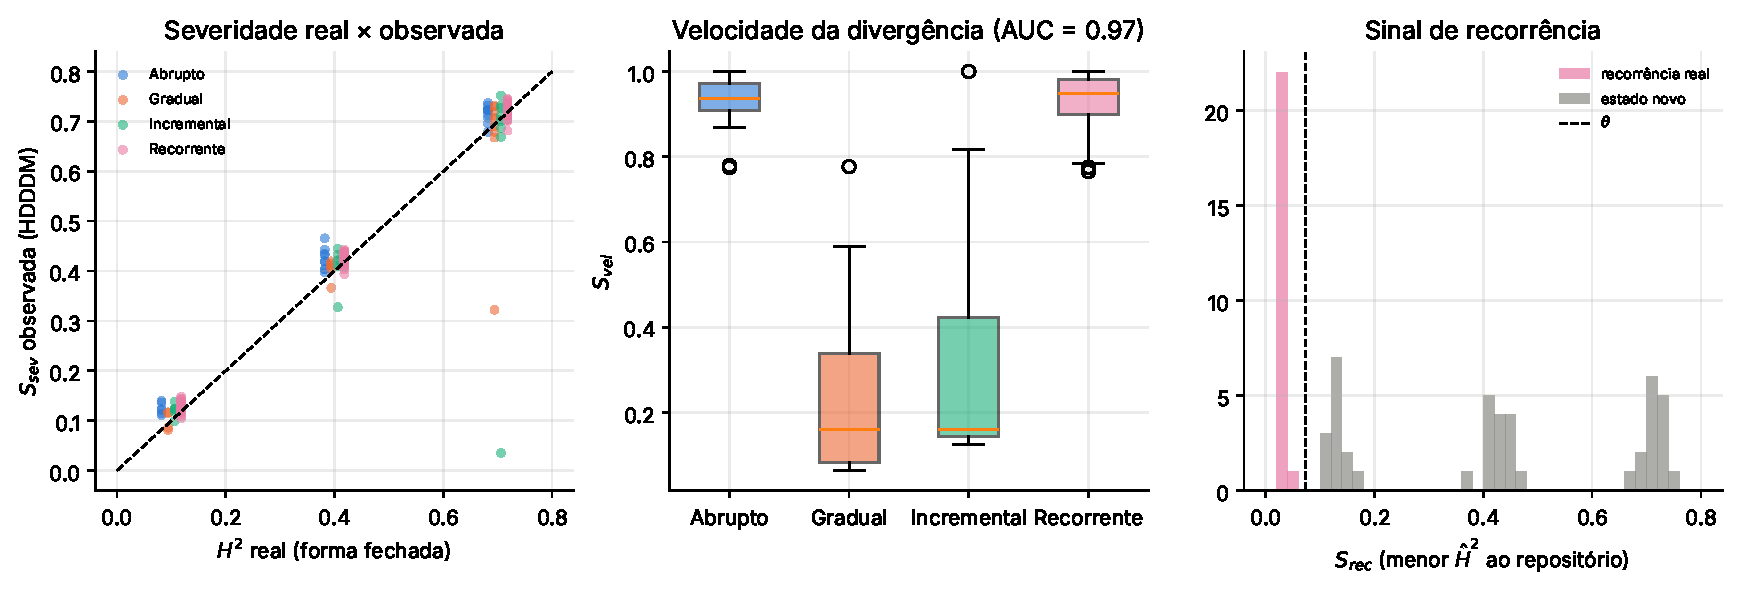
\includegraphics[width=\textwidth]{figuras/resultados/fig_sinais_observaveis.pdf}
\caption{Sinais observáveis do detector: severidade observada contra
severidade real (esquerda), velocidade da divergência por tipo de drift
(centro) e distância ao repositório nas transições para estados novos e nos
retornos a estados já vistos (direita).}
\label{fig:sinais}
\end{figure}

A severidade observada, medida no patamar após a detecção, acompanhou a
severidade real (Tabela~\ref{tab:severidade-obs}), com correlação de
Spearman de 0,897 e erro absoluto médio de 0,031. O viés foi pequeno nos
três níveis (de $-0{,}006$ a $+0{,}023$), mas a dispersão foi maior na
severidade alta (desvio-padrão de 0,111), por causa de transições lentas em
que o patamar ainda não havia sido atingido. Medida no próprio bloco da
detecção, a severidade observada subestimou a real nos níveis médio e alto
(0,337 e 0,499), justamente porque, nos padrões lentos, a detecção ocorre no
meio da transição.

\begin{table}[htbp]
\centering
\small
\caption{Severidade real versus severidade observada pelo HDDDM}
\label{tab:severidade-obs}
\begin{adjustbox}{max width=\textwidth}
\begin{tabular}{lrrrrrr}
\toprule
Nível & $H^2$ real & $S_{sev}$ média & DP & Viés & $\hat H^2$ na detecção & n \\
\midrule
Baixa & 0,1 & 0,123 & 0,015 & 0,023 & 0,110 & 36 \\
Média & 0,4 & 0,420 & 0,021 & 0,020 & 0,337 & 49 \\
Alta & 0,7 & 0,694 & 0,111 & -0,006 & 0,499 & 51 \\
\bottomrule
\end{tabular}
\end{adjustbox}
\par\vspace{2pt}{\footnotesize Spearman $\rho$ = 0,897; erro absoluto médio = 0,031.}
\end{table}


A velocidade da divergência separou com clareza as mudanças abruptas das
lentas: a mediana de $S_{vel}$ foi de 0,94 no padrão abrupto e 0,95 no
recorrente, contra 0,16 no gradual e no incremental, e a área sob a curva ROC
para distinguir os dois grupos foi de 0,974. O sinal não distingue, porém, o
padrão gradual do incremental, que têm a mesma média esperada ao longo da
transição (Figura~\ref{fig:gradual_incremental}).

O sinal de recorrência teve precisão e revocação de 100\% entre as transições
detectadas: os 23 retornos a um estado já visto tiveram distância ao
repositório de no máximo 0,044, abaixo de $\theta$, e as 43 transições para
estados novos tiveram distância de no mínimo 0,11. A separação decorre da
construção do padrão recorrente, em que estados distintos estão sempre a uma
distância igual à severidade da condição.

\subsection{Orientação preliminar}

Na validação cruzada entre sementes, o limiar de velocidade estimado no
treino foi $\tau_v = 0{,}82$, e os cortes de severidade observada, 0,271 e
0,554. A tabela de recomendação resultante indicou a janela deslizante para todo
o grupo gradual/incremental e para as severidades baixa e média do grupo
abrupto; o reset completo ou a reativação para o drift abrupto de severidade
alta; e, no grupo recorrente, a reativação para a severidade média, a janela
para a alta e estratégias distintas por classificador para a baixa. Nas 60 streams de teste, os sinais identificaram corretamente o
grupo de tipo em 71,7\% dos casos e o nível de severidade em 81,7\%; em nove
streams, todas graduais ou incrementais, o detector não produziu nenhum
episódio, e a estratégia padrão (a janela deslizante, para os três
classificadores) foi aplicada.

A Tabela~\ref{tab:orientacao} compara as políticas de escolha. A política
baseada em sinais (0,860) superou com folga a prática de sempre aplicar o
reset completo (0,806; $p < 0{,}001$) e ficou próxima do oráculo que conhece o
tipo e a severidade reais (0,863), embora a diferença para este tenha sido
significativa ($p = 0{,}036$). Ela não se distinguiu, porém, da política
fixa de sempre aplicar a janela deslizante (0,861; $p = 0{,}187$). Das 180
recomendações de teste, 136 foram a própria janela. Nas streams recorrentes,
onde as recomendações mais se afastaram da janela, a política baseada em
sinais (0,839) ficou abaixo tanto da janela (0,846) quanto do oráculo
(0,853).

\begin{table}[htbp]
\centering
\small
\caption{Acurácia das políticas de escolha de estratégia nas repetições de teste}
\label{tab:orientacao}
\begin{tabular}{lrrr}
\toprule
Política & Acurácia pós-drift & Perda vs. retrospecto & $p$ (vs. sinais) \\
\midrule
Sinais observáveis (proposta) & 0,860 & 0,009 & -- \\
Oráculo (tipo e severidade reais) & 0,863 & 0,006 & 0,036 \\
Sempre janela deslizante & 0,861 & 0,008 & 0,187 \\
Sempre reset & 0,806 & 0,064 & $<$ 0,001 \\
Sem retreinamento & 0,657 & 0,212 & -- \\
Melhor em retrospecto & 0,869 & 0,000 & -- \\
\bottomrule
\end{tabular}
\par\vspace{2pt}{\footnotesize 60 streams de teste $\times$ 3 classificadores; $p$: teste de Wilcoxon pareado contra a política baseada em sinais.}
\end{table}

